%\input{capitulos/resultados}
\chapter[Resultados e Discussões]{Resultados e Discussões}
\label{cap_Resultados e Discussoes}

    A presente seção tem por objetivo expor e avaliar os resultados obtidos a partir dos testes com o protótipo. Serão discutidos dados referentes a exatidão, tempo de medida e capacidade do sistema, sendo indicados os parâmetros utilizados. Ao final serão feitas considerações quanto aos dados obtidos.


\section{Resultados dos testes do protótipo}
\label{sec_Resultados dos testes do prototipo}

    Para avaliar o modelo proposto, foram testadas posições diferentes do sensor e das bagagens, sendo observados os resultados com malas deitadas, de lado, em pé e na diagonal, separadamente. Cada mala na determinada posição foi medida 10 vezes, reunindo nos resultados as médias desses valores. Inclusive, a questão das posições é citada como ponto em aberto nos trabalhos da revisão. Os testes foram realizados utilizando o Roi de 5 cm, capturando dados a um passo de 5 cm.

\subsection{Testes com sensor em diferentes posições}
\label{sec_Testes com sensor em diferentes posições}


    Para validar qual o ponto de melhor exatidão do sensor no protótipo, foram realizados testes em diferentes posições. Desse modo, foram selecionadas 3 alturas para testar com o sensor, sendo elas 1 m, 1,25 m e 1,50 m. A discussão quanto a altura e posição do sensor também foi observada como ponto em aberto nos trabalhos da Seção \ref{sec_Trabalhos relacionados}.
    
    Cada altura foi testada com uma mala deitada e em pé, ambas na horizontal. Para cada altura foram retiradas 10 medidas e calculadas as médias dos valores. As malas são mostradas nos testes de número 1 das Figuras \ref{fig:Malas_Deitadas} e \ref{fig:Malas_Em_Pe}, já a Tabela \ref{tab:testesDiferetesAlturasSensor} mostra o erro absoluto médio (MAE) retornado para as medidas. Os campos da tabela são Largura (L), Altura (A), Profundidade (P) e o tempo de medida (TM).


\begin{table}[h!]
\centering
\resizebox{\textwidth}{!}{%
\begin{tabular}{@{}ccccccc@{}}
\toprule
N & Altura do Sensor (m) & L (cm) & A (cm) & P (cm) & MAE  & TM (s) \\ \midrule
1 & 1          & 1,305  & 0,42   & 0,77   & 0,83 & 2,7    \\
2 & 1,25       & 2,715  & 3,34   & 0,195  & 2,08 & 2,05   \\
3 & 1,50       & 7,035  & 0,895  & 2,735  & 3,56 & 1,44   \\ \bottomrule
\end{tabular}%
}
\caption{exatidão do protótipo para alturas diferentes do sensor}
\label{tab:testesDiferetesAlturasSensor}
\end{table}

    Pela análise dos dados da Tabela \ref{tab:testesDiferetesAlturasSensor}, é possível perceber algumas diferenças importantes. Primeiro o menor MAE foi para a altura de 1 m (0,83 cm) indicando que essa posição retorna um resultado geral melhor, sendo que também é a altura mínima para o uso com malas de mão e de porão. Ainda, os erros de L incrementaram a cada teste chegando a 7,035 cm, já as dimensões A e P, tiveram os piores resultados nas alturas 1,25 m e 1,50 m. Sendo assim, os dados indicam que existe um erro de acuraria ligado a distância do sensor, sugerindo que, para o presente protótipo, uma proximidade de 1 m do sensor com a base da esteira gera menores erros.
    
    Outra informação observada é o decréscimo no tempo de medida. O tempo no teste 1 foi de 2,7 s até o mínimo de 1,44 s no teste 3 com altura de 1,50 m que teve o pior MAE. Por tanto, a exatidão está inversamente relacionada à altura que está diretamente relacionada à velocidade. Isso indica que é possível ajustar a posição do sensor para cenários onde a tolerância de erro é maior, obtendo assim, resultados mais rápidos.
    
    Quanto ao modelo final da presente pesquisa, é preferível ter a melhor exatidão possível para evitar transtornos e perdas financeiras. Por tanto, a altura selecionada como padrão para o protótipo foi de 1 m, visto que, nesse escopo, existe maior tolerância para o tempo do que para a exatidão.



\subsection{Testes com malas em posição deitada}
\label{sec_Testes com mala em posicao deitada}

    Os primeiros testes realizados foram com as malas em posição deitada. A Figura \ref{fig:Malas_Deitadas} mostra as malas utilizadas nos testes e a Tabela \ref{tab:Resultado da precisão do protótipo, malas deitadas} os resultados obtidos. Para cada bagagem foram coletadas 10 medidas e a partir disso foi calculada a média entre os valores. Os campos marcados com (R) são os valores reais e os campos marcados com (K) os valores retornados pelo sistema. A coluna N representa o código identificador da bagagem em questão. Os dados estão em termos de largura (L), altura (A), profundidade (P) e volume (V).

        \begin{figure}[h]
           \centering
           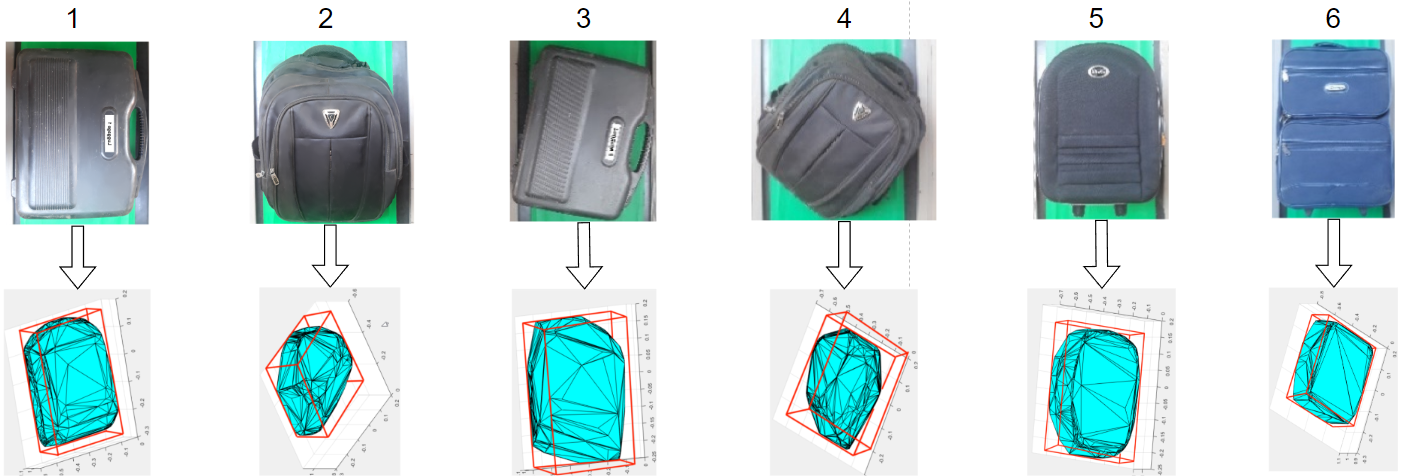
\includegraphics[width=0.8\textwidth]{imagens/imagens_tabelas/resultadosMalasDeitadas/Malas_Deitadas.png} 
           \caption{Testes Com malas deitadas (convex hull e OMBB)}
           \label{fig:Malas_Deitadas}
        \end{figure}


    
\begin{table}[h!]
\centering
\resizebox{\textwidth}{!}{%
\begin{tabular}{@{}llllllllllll@{}}
\toprule
N & L (R) cm & A (R) cm & P (R) cm & V(R) m3 & L(K)cm & A (K) cm & P(K) cm & V(K) m3 & MAE \\ \midrule
1 & 42,50 & 50 & 17,80 & 0,037 & 42,58 & 50,24 & 17,35 & 0,0371 & 0,25 \\
2 & 42,10 & 55,23 & 18,50 & 0,043 & 42,60 & 56,98 & 19,65 & 0,0476 & 1,13 \\
3 & 42,50 & 50 & 17,80 & 0,037 & 42,50 & 48,81 & 17,25 & 0,036 & 0,58 \\
4 & 42,10 & 55,23 & 18,50 & 0,043 & 43,38 & 48,79 & 18,54 & 0,040 & 2,58 \\
5 & 37,30 & 51,80 & 20,10 & 0,038 & 38,97 & 52,88 & 19,76 & 0,040 & 1,03 \\
6 & 41,00 & 58,01 & 22,00 & 0,052 & 44,71 & 59,14 & 21,65 & 0,057 & 1,73 \\ \midrule
 & MAE médio &  &  &  & 1,21 & 1,97 & 0,48 & 0,003 & 1,22 \\ \bottomrule
\end{tabular}%
}
\caption{Resultado da exatidão do protótipo, malas deitadas}
\label{tab:Resultado da precisão do protótipo, malas deitadas}
\end{table}

    A partir da análise dos resultados da Tabela \ref{tab:Resultado da precisão do protótipo, malas deitadas}, é possível observar que, para a mala 1, posicionada horizontalmente, obteve-se um MAE de 0,25 cm. Já a mochila 2 obteve MAE de 1,13 cm. Tais erros podem ser gerados, para além da amostragem e posição da mala, por pontos levemente deslocados devido à reflexão do sensor ao colidir com a superfície da mala. Outro fator que corrobora com os erros é o material macio da mochila 2, materiais macios, sempre que manuseados, podem se deformar e alterar as dimensões. Como durante os testes a 2 foi reposicionada, os resultados se alterarão em cada amostra.
    
    Os testes 3 e 4 foram realizados com as bagagens rotacionadas na diagonal. Os erros retornados foram de 0,58 cm e 2,58 cm, respectivamente. Em comparação com os resultados obtidos em 1 e 2, houve um aumento, isso se deve ao tratamento exclusivo que o algoritmo tem que realizar ao considerar que a nuvem de pontos é rotacionada. Outro fator que afeta os resultados são os slices de amostra que, dado que a mala está rotacionada, podem gerar leves erros de deslocamento de pontos, como, por exemplo, serrilhados. 
    
    Os testes 5 e 6 retornaram MAE de 1,03 cm e 1,73 cm, respectivamente. O maior erro absoluto dessas medidas ocorreu para os valores de altura, 1,12 cm. Ao comparar os resultados de 5 e 6 com 1, é possível notar indícios de que o erro é cumulativo. Isso pode estar relacionado à etapa de amostragem e o passo definido ou à necessidade de tratamentos extras da \textit{point cloud}, como filtragem.


\subsection{Testes com malas em posição de pé}
\label{sec_Testes com mala em posição de pe}

A segunda etapa de testes consistiu em coletar as dimensões das bagagens em posição de pé. Os resultados são mostrados na Tabela \ref{tab:Resultado da preciso do prottipo malas de pe}. A Figura \ref{fig:Malas_Em_Pe} mostra as malas utilizadas e a visualização dos dados coletados.

        \begin{figure}[h]
           \centering
           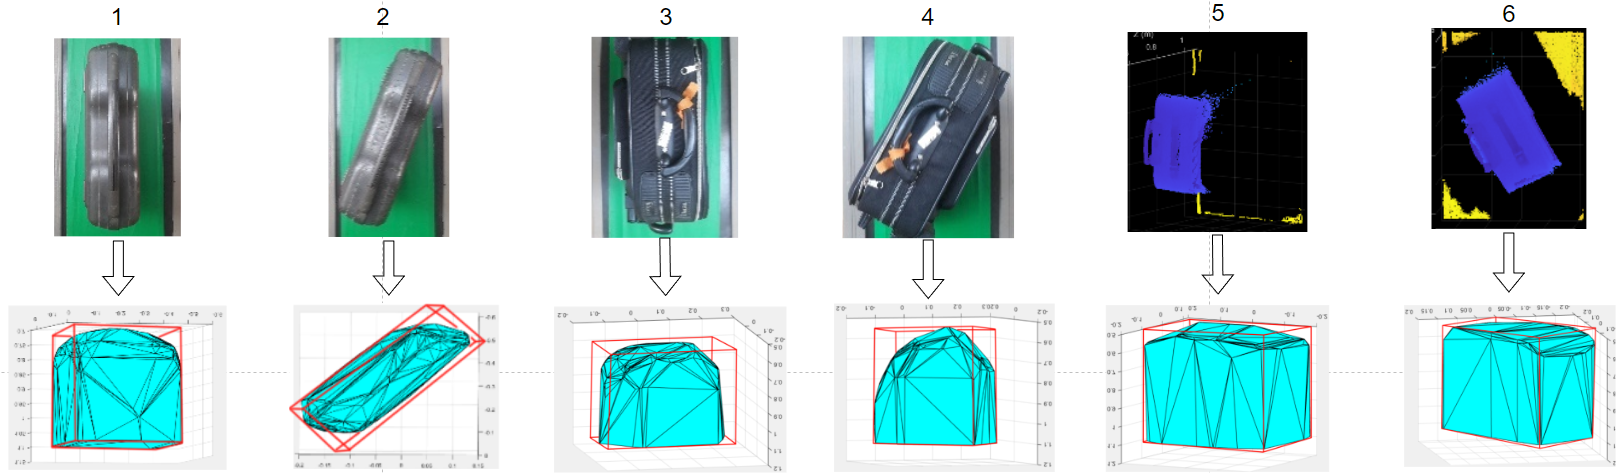
\includegraphics[width=0.8\textwidth]{imagens/imagens_tabelas/resultadosMalasEmPe/Malas_Em_Pe.png} 
           \caption{Testes com malas em pé (point cloud, convex hull e OMBB)}
           \label{fig:Malas_Em_Pe}
        \end{figure}


\begin{table}[h!]
\centering
\resizebox{\textwidth}{!}{%
\begin{tabular}{@{}llllllllll@{}}
\toprule
N & L (R) cm  & A (R) cm & P (R) cm & V(R) m3 & L(K)cm & A(K) cm & P(K) cm & V(K) m3 & MAE  \\ \midrule
1 & 42.50     & 50       & 17.80    & 0.037   & 39,97  & 49,40   & 18,89   & 0.0372  & 1,41 \\
2 & 42.50     & 50       & 17.80    & 0.037   & 39,95  & 52,89   & 19,09   & 0.0403  & 2,24 \\
3 & 37.30     & 51.80    & 20.10    & 0.038   & 36,45  & 54,81   & 23,58   & 0,047   & 2,45 \\
4 & 37.30     & 51.80    & 20.10    & 0.038   & 37,40  & 56,21   & 22,95   & 0.048   & 2,46 \\
5 & 41,00     & 58,01    & 22,00    & 0,052   & 38,82  & 59,66   & 25,33   & 0,058   & 2,39 \\
6 & 41.00     & 58.01    & 22.00    & 0.052   & 39,07  & 60,00   & 24,21   & 0.056   & 2,04 \\ \midrule
  & MAE médio &          &          &         & 1.69   & 2,43    & 2,4     & 0.005   & 2,16 \\ \bottomrule
\end{tabular}%
}
\caption{Resultado da exatidão do protótipo, malas de pé }
\label{tab:Resultado da preciso do prottipo malas de pe}
\end{table}


    O MAE total obtido para a mala de pé foi maior que o MAE das bagagens em posição deitada. A maior diferença foi o erro retornado na profundidade, sendo 1,92 cm a mais que o anterior. Isso é um indício de que a altura da bagagem pode influenciar na medida, provavelmente pelo topo estar mais próximo do kinect e existir diferenças na reflexão do IR.




\subsection{Testes com malas em posição de lado}
\label{sec_Testes com mala em posição de lado}

A terceira etapa de testes consistiu em coletar as dimensões das bagagens em posição de lado. Os resultados são mostrados na Tabela \ref{tab:Resultado da precisão do protótipo, malas de lado}. A Figura \ref{fig:Malas_DeLado} mostra as malas utilizadas e a visualização dos dados coletados. Nesse caso, a mala 1 e a mochila, não foram inclusas por não terem apoios de fábrica, para permanecerem nessa posição. 

        \begin{figure}[h]
           \centering
           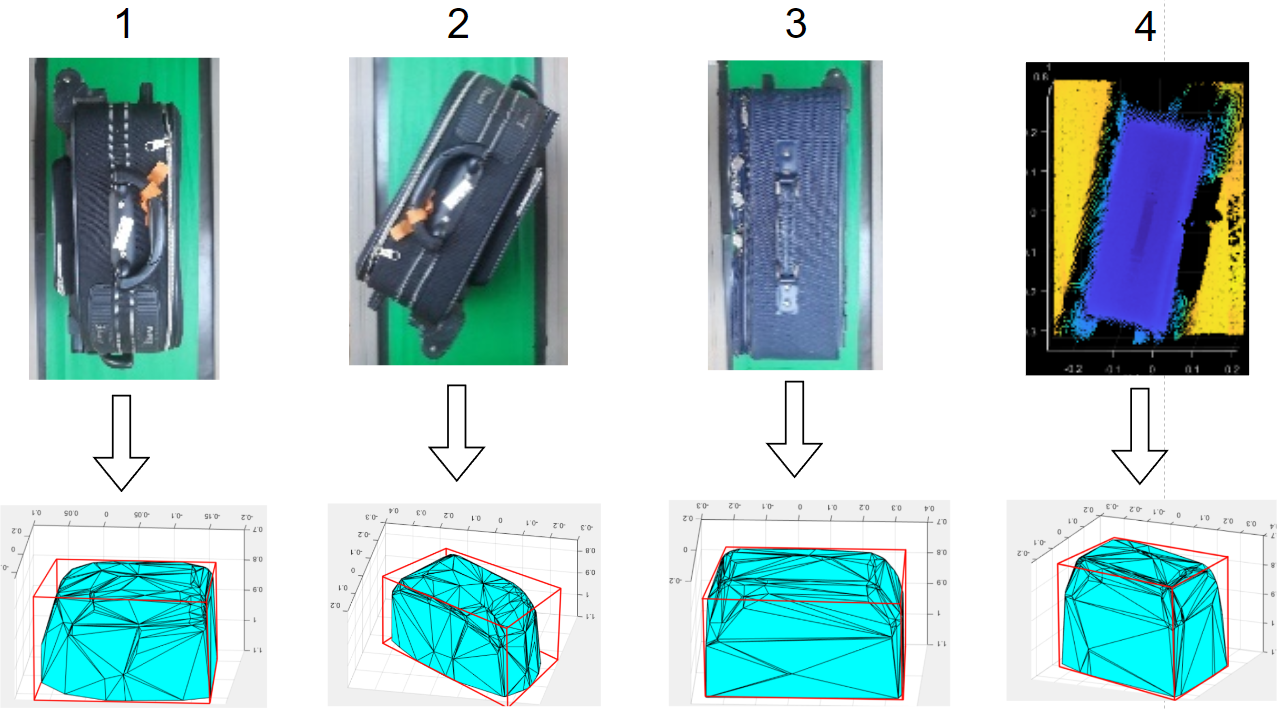
\includegraphics[width=0.5\textwidth]{imagens/imagens_tabelas/resultadosMalasDeLado/testes_Malas_de_lado.png} 
           \caption{Testes com malas de lado (\textit{point cloud}, convex hull e OMBB)}
           \label{fig:Malas_DeLado}
        \end{figure}


\begin{table}[h!]
\centering
\resizebox{\textwidth}{!}{%
\begin{tabular}{@{}llllllllll@{}}
\toprule
N & L (R) cm  & A (R) cm & P (R) cm & V(R) m3 & L(K)cm & A(K) cm & P(K) cm & V(K) m3 & MAE  \\ \midrule
1 & 37,30     & 51,80    & 20,10    & 0,038   & 35,36  & 50,34   & 24,97   & 0,044   & 2,76 \\
2 & 37,30     & 51,80    & 20,10    & 0,038   & 34,96  & 61,80   & 25,09   & 0,054   & 5,78 \\
3 & 41.00     & 58.01    & 22.00    & 0.052   & 39,22  & 62,79   & 30,24   & 0,074   & 4,93 \\
4 & 41.00     & 58.01    & 22.00    & 0.052   & 39,10  & 68,17   & 31,96   & 0,085   & 7,34 \\ \midrule
  & MAE médio &          &          &         & 1.99   & 6,6     & 7,01    & 0,012   & 5,20 \\ \bottomrule
\end{tabular}%
}
\caption{Resultado da exatidão do protótipo, malas de lado}
\label{tab:Resultado da precisão do protótipo, malas de lado}
\end{table}





\section{Discussão quanto aos resultados gerais}
\label{sec_Discussão quanto aos resultados gerais}

A Tabela \ref{tab:resulmoResultadoDiferetesPosicoes} resume os resultados dos erros retornados em centímetros. Os dados estão divididos por posição da bagagem, sendo o campo MAE total a média geral dos erros naquela posição.


\begin{table}[h!]
\centering
\resizebox{\textwidth}{!}{%
\begin{tabular}{@{}lccccc@{}}
\toprule
\textbf{Posição} &
  \multicolumn{1}{l}{\textbf{Largura (cm)}} &
  \multicolumn{1}{l}{\textbf{Altura (cm)}} &
  \multicolumn{1}{l}{\textbf{Profundidade (cm)}} &
  \multicolumn{1}{l}{\textbf{Volume ($m^3$)}} &
  \multicolumn{1}{l}{\textbf{MAE total}} \\ \midrule
Deitada & 1,21 & 1,97 & 0,48 & 0,003 & 1,22 \\
Em pé & 1,69 & 2,43 & 2,4  & 0,005 & 2,16 \\
De lado   & 1,99 & 6,6  & 7,01 & 0,012 & 5,20 \\ \midrule
Média   & 1,63 & 3,7  & 3,3  & 0,007 & 2,86 \\ \bottomrule
\end{tabular}%
}
\caption{Comparação dos MAEs em diferentes posições}
\label{tab:resulmoResultadoDiferetesPosicoes}
\end{table}

    Por meio da análise dos erros, é possível perceber que os melhores resultados são das medidas com malas deitadas. Em contraste, o pior resultado foi para a posição em pé. Nesse caso, dois pontos de atenção são os erros de comprimento e profundidade. Enquanto os erros de largura permaneceram uniformes, os outros aumentaram significativamente de uma posição para outra. Isso indica uma instabilidade quanto a essas medidas.
    
    Em relação ao comprimento, essa instabilidade pode ser advinda da amostragem. Isso se deve a quedas na taxa de quadros de captura do sensor kinect. Outro fator que contribui são alterações na velocidade da esteira no momento da medida, influenciada por aquecimentos, atritos e o peso das malas. Uma forma de amenizar esse problema é aumentar o torque do motor e melhorar o controle de velocidade.
    
    Quanto ao tempo gasto por medição, o sistema utiliza uma média de 0,14 s/cm. Isso significa que, por exemplo, dada uma mala com 80 cm de comprimento (a maior medida segundo a ANAC para bagagem de despacho), o sistema gastaria 11,8 s. Como o tempo de medição influencia diretamente no check-in, é interessante fazer melhorias no sistema, como, por exemplo, reduzir o tempo de máquina do algoritmo e aumentar a velocidade da esteira.
    
    Pelo levantamento dos resultados de todos os testes, o erro absoluto médio foi de 1,63 cm para largura, 3,7 cm para comprimento e 3,3 cm para profundidade, totalizando um erro absoluto médio de 2,86 cm. Sendo assim, o sistema tem potencial para ser utilizado na prática, especialmente se as bagagens forem dispostas com o mínimo de padronização. 

    
\section{Simulação de operação do modelo proposto}
\label{sec_Cenários simulados de operação do produto}

    Na presente seção, será discutido um cenário de testes de operação do modelo de medida de bagagens desenvolvido nessa pesquisa. Tal cenário consiste em uma simulação de processo de check-in utilizando dados reais, focado apenas no \textit{tempo de medida de bagagens}. Os cenários exploram sempre os piores casos, ou seja, são considerados os valores máximos para qualquer processo ou medida. Para fins de comparação, foram buscados dados com resultados ótimos indicados pela \citeonline{iata_2022_level} e outras pesquisas. Considerando que cada companhia aérea pode estabelecer os limites de peso e bagagem de acordo com suas próprias normas, foram levados em conta os parâmetros técnicos do modelo da aeronave. 

    Primeiramente, é fundamental destacar dois aspectos relacionados à operação de \textit{self bag drop} nas esteiras de atendimento: o posicionamento e a eficiência. Em relação ao posicionamento, optou-se pela abordagem \textit{two-step} conforme descrita na Seção \ref{subsec_Sensores a laser fixos e moveis}, uma vez que o foco principal é o tempo de medição. No que tange à eficiência, não foi identificada, durante a revisão, uma norma universal que estabeleça um tempo máximo. Isso pode variar significativamente devido às diferenças de tecnologia, capacidade e usabilidade. Contudo, é importante mencionar discussões, como a realizada por \citeonline{fte_2008_the}, que sugerem que, independentemente do posicionamento (seja "one-step" ou "two-step"), o processo de medição de bagagem pelo \textit{self bag drop} deve ser concluído em, no máximo, \textit{30s}, sendo o tempo ideal \textit{15s}.

    Dado as definições expostas, foi selecionada a aeronave A320 para o cenário, a mesma é ilustrada na Figura \ref{fig:a320Modelo}. A Tabela \ref{tab:definicoesTecnicasDaAeronave} reúne as principais definições da aeronave, tais informações foram retiradas do modelo técnico disponibilizado em \cite{anacargo_2023_a320321ana}. O A320 comporta até 150 passageiros, com capacidade de 25kg de bagagens de mão por pessoa com bagageiro para 104 bagagens. O porão é dividido em compartimento da frente, que suporta 3 contêineres somando até 3402kg e traz, que suporta 4 contêineres somando até 4536kg. O BULK, que é um compartimento para cargas em tamanho e forma fora do padrão, suporta até 1497kg \cite{anacargo_2023_a320321ana, airfrance_2019_air}.

        \begin{figure}[h]
           \centering
           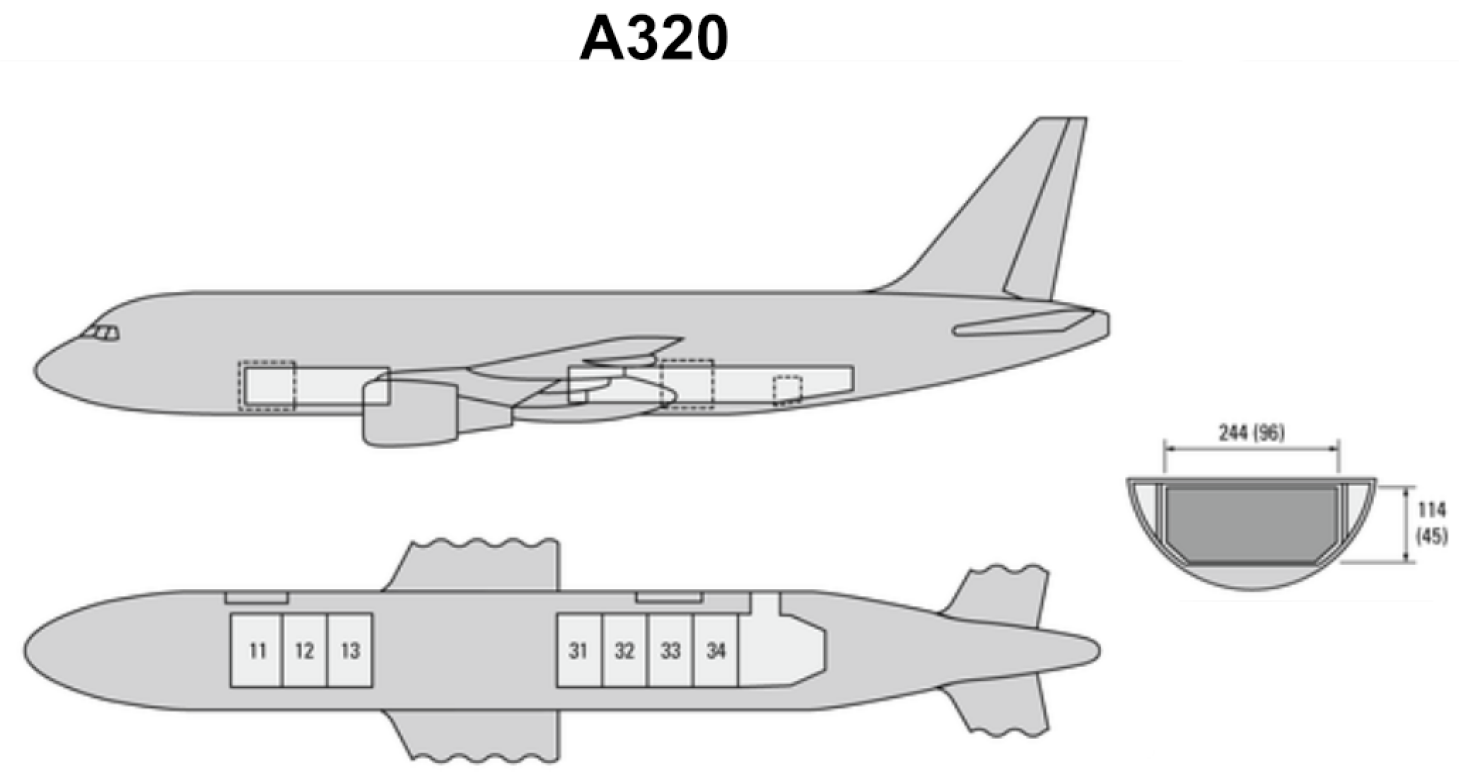
\includegraphics[width=0.7\textwidth]{imagens/a320Modelo.png} 
           \caption{Modelo técnico A320. Adaptado de \cite{anacargo_2023_a320321ana}}
           \label{fig:a320Modelo}
        \end{figure}


\begin{table}[h!]
\centering
\begin{tabular}{@{}lll@{}}
\toprule
\multicolumn{1}{c}{{Atributo}} & \multicolumn{1}{c}{{ Valor}} & \multicolumn{1}{c}{{Total}} \\ \midrule
Quantidade de passageiros total                 & 150                     &                                                                                           \\
                                                & Até 104 bagagens        &                                                                                           \\
\multirow{-2}{*}{Capacidade de bagagens de mão} & Até 25kg por passageiro &                                                                                           \\
                                                & Frente (FWD)            & \begin{tabular}[c]{@{}l@{}}3 containers\\ 3402kg\\ Aproximadamente 148 malas\end{tabular} \\
                                                & Trás (AFT)              & \begin{tabular}[c]{@{}l@{}}4 containers\\ 4536kg\\ Aproximadamente 197 malas\end{tabular} \\
\multirow{-3}{*}{Área do porão}                 & Bulk                    & 1497kg                                                                                    \\ \bottomrule
\end{tabular}
\caption{Definições técnicas da aeronave A320 \cite{anacargo_2023_a320321ana}}
\label{tab:definicoesTecnicasDaAeronave}
\end{table}
    
    Para compor o cenário, foram consideradas as recomendações quanto a bagagens descritas na Seção \ref{subsec_processo Processo de embarque}. Referente a quantidade, o estudo de \citeonline{appelt_2007_simulation} realizado no aeroporto internacional de Buffalo Niagara, indicou que em média se tem 1,61 bagagens por passageiro, considerando, também, as recomendações da ANAC, até duas bagagens (uma de mão e uma de despacho), não são taxadas. Dessa forma, foram contabilizadas uma bagagem de mão e uma de despacho por passageiro. 

    Tendo definidas as quantidades de bagagens, para parametrizar a eficiência ótima dos processos aeroportuários, foi utilizado o \textit{benchmark} gerado pela \citeonline{iata_2022_level}. O foco dessa pesquisa é o processo de check-in, desse modo a Figura \ref{fig:tempoDeCheckinSegundoANAC} indica os tempos ótimos dessa etapa segundo a IATA. Cabe destacar que, o benchmark não se restringe apenas a aeroportos com \textit{self bag drop}, logo, os dados são gerais. Com isso, tem-se que o tempo adequado para check-in, que inclui a etiquetagem e medida de bagagens, é de no máximo 7 minutos. Nos cálculos foram considerados apenas o tempo de medida da bagagem, que pode levar até 5 minutos. 

        \begin{figure}[h!]
           \centering
           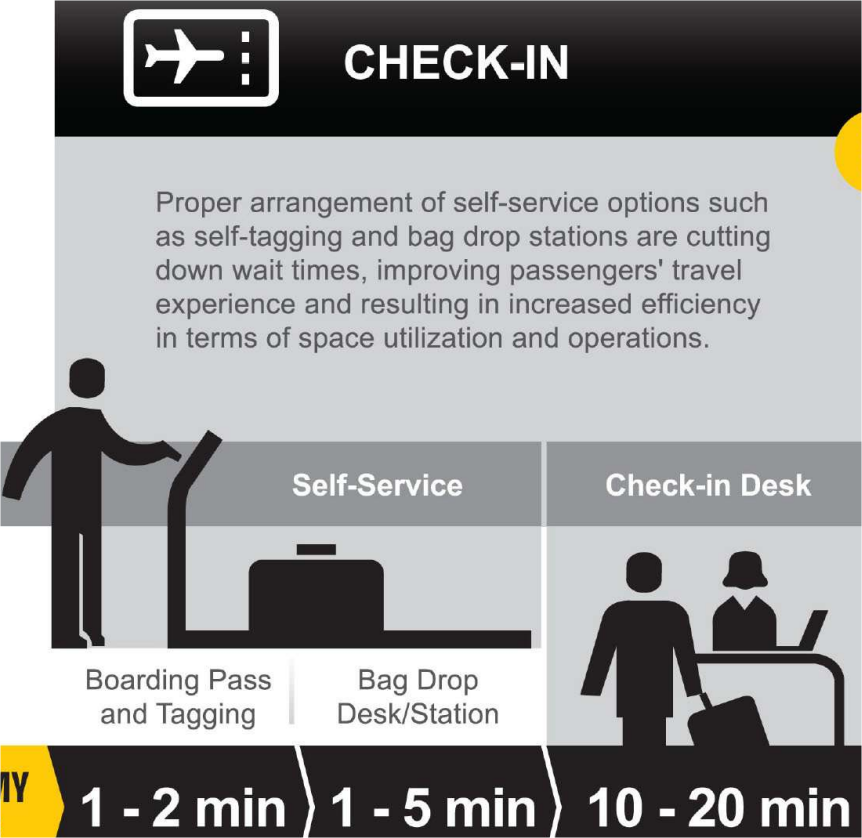
\includegraphics[width=0.5\textwidth]{imagens/tempoDeCheckinSegundoANAC.png} 
           \caption{Benchmark processo de check-in. Adaptado de \cite{iata_2022_level}}
           \label{fig:tempoDeCheckinSegundoANAC}
        \end{figure}

    Outra informação considerada, é o tempo médio máximo de check-in, esse dado varia entre as companhias e voos. Algumas recomendações orientam que é apropriado realizar check-in com 30 a 60 minutos de antecedência ao tempo de embarque, que, para uma aeronave como o A320, pode chegar a 30 minutos. Nesse contexto, o processo todo duraria até 90 minutos \cite{universityofminnesota_2022_airport, anac_2016_anac}. Na prática, é possível fazer check-in online, nos kiosks e nas filas de atendimento, contudo, para esse cenário, é considerado que todos os passageiros realizaram check-in nas filas utilizando as esteiras, todos dentro do prazo máximo de 60 minutos. 

    Baseado nessa informação, foi realizado o dimensionamento da quantidade de esteiras em paralelo necessárias para cumprir o tempo limite. A Tabela \ref{tab:Dimensionamento da operao do modelo proposto em comparao com diferentes mtricas de mercado} mostra os resultados, é importante reiterar que foi considerado apenas o tempo de medida de bagagens. Os dados indicam que 1 esteiras foi suficientes para cumprir o prazo de 60 minutos considerando a operação com o tempo ótimo para \textit{self bag drop}. Para o modelo dessa pesquisa, 1 esteira também foi suficiente, mas comparado ao tempo ótimo, seriam necessárias 2 esteiras para ter desempenho semelhante. Já o tempo máximo para \textit{self bag drop} necessitou de 2 esteiras para não ultrapassar o limite. As demais métricas não alcançaram o objetivo, para a projeção média da IATA seriam necessárias 7 esteiras e para as recomendações máximas de \textit{self bag drop} seriam necessárias 4. 

\begin{table}[h!]
\centering
\resizebox{\textwidth}{!}{%
\begin{tabular}{llllll}
\hline
Tipo de abordagem &
  \begin{tabular}[c]{@{}l@{}}Quantidade \\ de passageiros\end{tabular} &
  \begin{tabular}[c]{@{}l@{}}Tempo gasto \\ de medida por \\ passageiro (s)\end{tabular} &
  \begin{tabular}[c]{@{}l@{}}Tempo gasto\\ total com check-in\\ utilizando \\ 1 esteira(h)\end{tabular} &
  \begin{tabular}[c]{@{}l@{}}Tempo gasto \\ total com check-in\\ utilizando \\ 2 esteiras(h)\end{tabular} &
  \begin{tabular}[c]{@{}l@{}}Tempo gasto \\ total com check-in\\ utilizando\\  3 esteiras (h)\end{tabular} \\ \hline
\begin{tabular}[c]{@{}l@{}}Projeção da IATA \\ (máximo)\end{tabular}            & 150 & 300 & 12,5 & 6,3  & 4,17 \\
\begin{tabular}[c]{@{}l@{}}Projeção da IATA\\ (médio)\end{tabular}              & 150 & 150 & 6,3  & 3,15 & 2,1  \\
\begin{tabular}[c]{@{}l@{}}Recomendações \\ self-bag-drop (máximo)\end{tabular} & 150 & 30  & 1,25 & 0,63 & 0,42 \\
\begin{tabular}[c]{@{}l@{}}Recomendações \\ self-bag-drop (ótimo)\end{tabular}  & 150 & 15  & 0,63 & 0,32 & 0,21 \\
Produto dessa pesquisa                                                          & 150 & 19  & 0,80 & 0,4  & 0,27 \\ \hline
\end{tabular}%
}
\caption{Dimensionamento da operação do modelo proposto em comparação com diferentes métricas de mercado para aeronave A320}
\label{tab:Dimensionamento da operao do modelo proposto em comparao com diferentes mtricas de mercado}
\end{table}


    Os dados demonstram que, a solução proposta se aproxima dos resultados ótimos, sugerindo a necessidade de melhorias. Comparando os preços dos dispositivos de sef bag drop do mercado com os sensores de profundidade, utilizado no produto dessa pesquisa, se tem maior economia direta utilizando 2 esteiras com os sensores de profundidade do que comprando 1 esteiras com o dispositivo do mercado. Cabe recapitular que esse é um cenário simulado, que desconsidera dados dinâmicos e aleatórios, contudo, ele indica que o produto dessa pesquisa tem potencial de ser aplicado na prática. 




\begin{comment}

\section{Próximos passos da pesquisa}
\label{sec_Proximos passos da pesquisa}


    A presente seção expõe o planejando quanto as próximas etapas da pesquisa. Até então, foram discutidos neste trabalho os resultados obtidos quanto as fases de revisão sistemática, prototipagem e o primeiro conjunto de testes. Algumas informações previstas no Capítulo \ref{cap_Materiais e Metodos}, já foram abordados ao todo ou de maneira introdutória, como, por exemplo, avaliações quanto as possíveis posições da bagagem, tempo de medida e exatidão do sensor. Desse modo, a Tabela \ref{tab:Cronograma de prximos passos da pesquisa} expõe o planejamento dos próximos passos desta pesquisa conforme o tempo. 



\begin{table}[h!]
\centering
\resizebox{\textwidth}{!}{%
\begin{tabular}{ll|cc|ccc}
 &
   &
  \multicolumn{2}{c|}{2022} &
  \multicolumn{1}{l}{} &
  \multicolumn{1}{l}{2023} &
  \multicolumn{1}{l}{} \\ \hline
\multicolumn{1}{|c|}{ID} &
  \multicolumn{1}{c|}{Passo/Ação} &
  \multicolumn{1}{c|}{Nov.} &
  Dez. &
  \multicolumn{1}{c|}{Jan.} &
  \multicolumn{1}{c|}{Fev.} &
  \multicolumn{1}{c|}{Mar.} \\ \hline
\multicolumn{1}{|l|}{1} &
  Apresentação de exame de qualificação &
  \multicolumn{1}{c|}{X} &
   &
  \multicolumn{1}{c|}{} &
  \multicolumn{1}{c|}{} &
  \multicolumn{1}{c|}{} \\ \hline
\multicolumn{1}{|l|}{2} &
  Testes com mais posições do sensor &
  \multicolumn{1}{c|}{} &
  X &
  \multicolumn{1}{c|}{} &
  \multicolumn{1}{c|}{} &
  \multicolumn{1}{c|}{} \\ \hline
\multicolumn{1}{|l|}{3} &
  Testes com bagagens em formato fora do padrão &
  \multicolumn{1}{c|}{} &
  X &
  \multicolumn{1}{c|}{X} &
  \multicolumn{1}{c|}{} &
  \multicolumn{1}{c|}{} \\ \hline
\multicolumn{1}{|l|}{4} &
  Avaliação quanto a exatidão do protótipo &
  \multicolumn{1}{c|}{} &
  X &
  \multicolumn{1}{c|}{X} &
  \multicolumn{1}{c|}{} &
  \multicolumn{1}{c|}{} \\ \hline
\multicolumn{1}{|l|}{5} &
  Avaliação quanto a dificuldades na implementação &
  \multicolumn{1}{c|}{} &
  X &
  \multicolumn{1}{c|}{X} &
  \multicolumn{1}{c|}{} &
  \multicolumn{1}{c|}{} \\ \hline
\multicolumn{1}{|l|}{6} &
  Avaliação quanto a complexidade de incorporar o sensor &
  \multicolumn{1}{c|}{} &
  X &
  \multicolumn{1}{c|}{X} &
  \multicolumn{1}{c|}{} &
  \multicolumn{1}{c|}{} \\ \hline
\multicolumn{1}{|l|}{7} &
  Envio de um artigo sobre o trabalho para uma revista &
  \multicolumn{1}{c|}{} &
   &
  \multicolumn{1}{c|}{X} &
  \multicolumn{1}{c|}{X} &
  \multicolumn{1}{c|}{} \\ \hline
\multicolumn{1}{|l|}{8} &
  Inserção de códigos desenvolvidos nos apêndices do trabalho &
  \multicolumn{1}{c|}{} &
   &
  \multicolumn{1}{c|}{} &
  \multicolumn{1}{c|}{X} &
  \multicolumn{1}{c|}{} \\ \hline
\multicolumn{1}{|l|}{9} &
  Finalização do modelo proposto, dados dos testes e documentação &
  \multicolumn{1}{c|}{} &
   &
  \multicolumn{1}{c|}{} &
  \multicolumn{1}{c|}{X} &
  \multicolumn{1}{c|}{X} \\ \hline
\multicolumn{1}{|l|}{10} &
  Realização da defesa do produto final &
  \multicolumn{1}{c|}{} &
   &
  \multicolumn{1}{c|}{} &
  \multicolumn{1}{c|}{} &
  \multicolumn{1}{c|}{X} \\ \hline
\end{tabular}%
}
\caption{Cronograma de próximos passos da pesquisa}
\label{tab:Cronograma de prximos passos da pesquisa}
\end{table}



Na atividade 1 será construído um gráfico comparativo entre as tecnologias de mercado e o modelo proposto, avaliando custo, tempo, exatidão e segurança. Nas atividades 2 e 3 serão realizados testes com mais posições do sensor e bagagens em outros formatos (Ex. malas de instrumentos). Nos passos 4, 5 e 6, serão realizadas avaliações quanto aos dados dos testes, validando, por exemplo, exatidão, tempo, dificuldades de implementação/incorporação do sensor.  Os passos 7 e 8, correspondem a qualificação e envio de um artigo a uma revista a ser definida. Nas ações 9 e 8, será finalizado os detalhes do produto final e da documentação. E, finalmente, na atividade 11, será realizada a defesa do produto final.


\end{comment}
